\chapter{La Blockchain}
Una volta che le transazioni vengono create e firmate tramite la logica degli script, esse devono essere raggruppate e "sigillate" all'interno di un \textbf{blocco}. 
La blockchain non è altro che una catena sequenziale di questi contenitori, dove ogni blocco garantisce l'immutabilità dei dati che contiene.
\section{Il Blocco}
Ogni blocco è identificato da un \textbf{Header} (intestazione), che possiamo immaginare come la carta d'identità del blocco stesso. Esso contiene i metadati fondamentali per la sicurezza della rete:
\begin{itemize}
    \item \textbf{Hash del blocco precedente (\textit{prev\_block}):} È il legame che crea la catena. Ogni blocco contiene l'impronta digitale di quello precedente; se qualcuno provasse a modificare una transazione in un blocco passato, l'hash cambierebbe, rendendo istantaneamente invalidi tutti i blocchi successivi.
    \item \textbf{Nonce e Bits:} Sono parametri legati al mining. Il \textit{nonce} è il numero che i miner continuano a variare per trovare un hash che soddisfi la difficoltà della rete (\textit{bits}), confermando così il blocco tramite la Proof-of-Work.
    \item \textbf{Merkle Root (\textit{mrkl\_root}):} Una stringa che riassume in modo univoco tutte le transazioni presenti nel blocco
\end{itemize}
    
\subsection{Merkle Tree e Proof of Membership}
Per gestire i dati delle transazioni in modo efficiente, Bitcoin non le elenca semplicemente una dopo l'altra, ma utilizza una struttura chiamata \textbf{Merkle Tree} (albero di Merkle). Si tratta di un albero binario in cui si parte dagli hash delle singole transazioni alla base e, accoppiandoli, si sale di livello calcolando nuovi hash fino ad arrivare alla radice (\textbf{Merkle Root}).
Questa struttura è fondamentale per la cosiddetta \textbf{Proof of Membership}. Supponiamo che un utente $A$ utilizzi un wallet "leggero" sul suo smartphone. Grazie al Merkle Tree, $A$ non deve scaricare tutte le migliaia di transazioni del blocco, ma gli basta ricevere solo una piccola serie di hash intermedi. Combinando questi hash con quello della propria transazione, $A$ può ricalcolare la Merkle Root: se il risultato coincide con quello presente nell'header del blocco, allora ha la certezza matematica che la sua transazione è stata confermata.Infatti, non tutti i partecipanti alla rete scaricano l'intera blockchain. Esistono due tipologie di nodi:
\begin{itemize}
    \item \textbf{Full Node:} Sono i nodi che contengono l'intera cronologia delle transazioni e verificano ogni singola regola del protocollo. Sono "pesanti" in termini di memoria ma garantiscono la massima sicurezza. I miner possono solamente essere dei nodi di questo tipo.
    \item \textbf{Lightweight Node (o nodi SPV):} Sono nodi che non contengono tutte le transazioni, bensì conservano solo i \textbf{Block Header}. Quando questi nodi hanno necessità di verificare l'esistenza di una certa transazione, interrogano i Full Node chiedendo loro di inviargli i dati necessari (il "cammino" nell'albero di Merkle) per effettuare la Proof of Membership.
\end{itemize}
\subsection{Coinbase transaction}
Fino ad ora abbiamo visto come $A$ possa inviare Bitcoin a $B$ partendo da fondi già esistenti (UTXO). Ma come entrano in circolazione i nuovi Bitcoin se non esiste una banca centrale? La soluzione è la \textbf{Coinbase Transaction}, una transazione "speciale" che deve essere presente obbligatoriamente come prima operazione di ogni singolo blocco. Questa transazione ha tre caratteristiche fondamentali:
\begin{itemize}
    \item \textbf{Emissione Monetaria:} È l'unico modo previsto dal protocollo per \textbf{creare nuovi Bitcoin}. Non avendo un input che proviene da una transazione precedente, essa "genera" valuta dal nulla seguendo una regola matematica precisa.
    \item \textbf{Remunerazione dei Miner:} Rappresenta il guadagno principale per chi mette in sicurezza la rete. Il miner che riesce a chiudere il blocco assegna a se stesso una somma composta da:
    \begin{enumerate}
        \item Il \textbf{Block Subsidy} (il premio per il blocco).
        \item Le \textbf{Fees} (le commissioni) di tutte le transazioni incluse nel blocco.
    \end{enumerate}
    Il premio iniziale era di 50 BTC, ma ogni 210.000 blocchi (circa 4 anni) questa cifra viene dimezzata tramite un evento chiamato \textbf{Halving}. Come si vede nell'immagine, nel 2020 il premio è sceso a 6.25 BTC e dall'aprile 2024 è passato a \textbf{3.125 BTC}.
    
    \item \textbf{Il campo Coinbase:} A differenza delle transazioni normali, l'input della Coinbase Transaction non punta a un UTXO precedente (infatti il campo \textit{hash} è composto da soli zeri). Al suo posto troviamo un campo libero chiamato \textit{coinbase}, dove il miner può inserire dati arbitrari. L'esempio più famoso è quello di Satoshi Nakamoto nel Blocco 0, dove inserì il titolo del quotidiano \textit{The Times} per denunciare l'instabilità del sistema bancario tradizionale.
\end{itemize}

\section{Il Network Bitcoin}
Dopo aver analizzato la struttura dei blocchi, è fondamentale capire come le informazioni (transazioni e blocchi) viaggino tra i partecipanti. Bitcoin non si appoggia a un server centrale, ma utilizza una rete \textbf{P2P ad-hoc} dove tutti i nodi sono considerati uguali.

La rete Bitcoin presenta alcune proprietà fondamentali che ne garantiscono la resilienza:
\begin{itemize}
    \item \textbf{Connessioni TCP:} I nodi comunicano solitamente sulla porta \texttt{8333}.
    \item \textbf{Topologia Logica vs Fisica:} La rete è organizzata in modo "random". Un nodo in Italia potrebbe essere logicamente connesso a un nodo in Giappone; la struttura logica non rispecchia quella geografica.
    \item \textbf{Discovery e Oblivion:} Quando un nuovo nodo entra nella rete (come il nodo 8 nell'immagine), deve "scoprire" i suoi vicini. Lo fa inviando messaggi di \textit{getaddr()} per ottenere liste di indirizzi IP di altri nodi attivi. Allo stesso modo, se un nodo smette di rispondere, viene dimenticato dalla rete (\textit{oblivion}).
\end{itemize}
\begin{figure}[H]
    \centering
    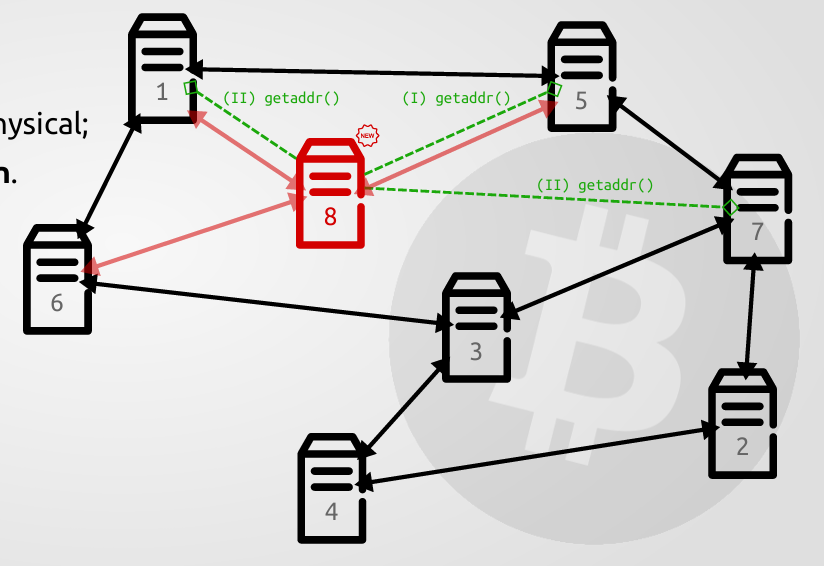
\includegraphics[width=0.7\linewidth]{Images/capitolo_mdr_2/nuovo_nodo.png}
\end{figure}

\subsection{Gossip Protocol}
Quando un utente $A$ crea una transazione per pagare $B$, questa non finisce immediatamente nella blockchain. Deve prima essere propagata a tutti i nodi della rete tramite un \textbf{Gossip Protocol} (o \textit{Flooding}).
Il funzionamento è simile al diffondersi di un pettegolezzo: $A$ invia la transazione ai propri vicini, questi la verificano e, se valida, la inviano ai propri vicini, e così via fino a coprire l'intera rete in pochi secondi.
\subsection*{La Transaction Pool e i Controlli Standard}
Ogni singolo nodo mantiene in memoria una "vasca" temporanea chiamata \textbf{Transaction Pool} (o \textit{Mempool}), dove conserva le transazioni ricevute che sono in attesa di essere inserite in un blocco dai miner. Prima di accettare una transazione nella propria pool e inoltrarla agli altri, ogni nodo effettua dei \textbf{controlli standard}:
\begin{enumerate}
    \item \textbf{Validità:} La transazione deve avere firme corrette e formattazione valida.
    \item \textbf{Script Whitelist:} Lo script deve rientrare tra quelli considerati "standard".
    \item \textbf{Unicità:} La transazione non deve essere già presente nella pool.
    \item \textbf{Assenza di conflitti:} La transazione non deve tentare di spendere UTXO già impegnati da altre transazioni presenti nella pool (evitando il double spending immediato).
\end{enumerate}

Poiché la rete è distribuita e la propagazione richiede tempo, le Mempool dei vari nodi non sono sempre identiche (\textit{out-of-sync}). 
Se due transazioni in conflitto (ad esempio $A$ prova a mandare gli stessi soldi sia a $C$ che a $B$ contemporaneamente) si diffondono nella rete, si crea una \textbf{Race Condition}. 
In questo caso vale la regola del \textbf{"the first win!"}: ogni nodo terrà in memoria solo la prima transazione che riceve e scarterà la seconda. Sarà poi il miner, scegliendo quale includere nel prossimo blocco, a decretare quale delle due transazioni diventerà definitiva. Esiste però un'eccezione chiamata \textbf{Replace-By-Fee (RBF)}, che permette a un utente di "sovrascrivere" una propria transazione in attesa con una nuova che offra una mancia (\textit{fee}) più alta ai miner.

\subsection{Propagazione dei Blocchi}
Allo stesso modo di come funziona la diffusione di nuove transazioni, avviene la propagazione dei nuovi blocchi.

QUi i controlli sono di diverso tipo, un blocco viene inoltrato solo se:
\begin{itemize}
    \item È stato risolto il \textbf{puzzle crittografico}.
    \item Contiene solo \textbf{transazioni valide}.
    \item È costruito sulla \textbf{catena più lunga} evitando, così, fork.
\end{itemize}

Quando un miner scopre un nuovo blocco valido, lo trasmette immediatamente ai suoi peer. Ogni nodo che lo riceve verifica la sua validità e, se soddisfa tutti i requisiti, lo inoltra ai propri peer e lo aggiunge alla propria copia locale della blockchain. Questo meccanismo di propagazione a cascata garantisce che i blocchi validi si diffondano rapidamente attraverso l'intera rete.

Questi controlli assicurano che solo blocchi legittimi vengano incorporati nella blockchain, prevenendo attacchi e divergenze non intenzionali.

\subsection{Tipologie di Nodi}
Come già accennato precedentemente esistono due tipi di nodi:
\begin{itemize}
    \item I \textbf{Full Nodes};
    \item I \textbf{Lightweight Node};
\end{itemize}

Per quanto riguarda i full node, questi possiedono le seguenti caratteristiche:
\begin{itemize}
    \item \textbf{Connettività permanente}: Mantengono una presenza costante nella rete per massimizzare la resilienza del sistema.
    \item \textbf{Archiviazione completa}: Conservano l'intera blockchain, comprensiva di tutte le transazioni dalla genesi (circa 460 GB nel 2023).
    \item \textbf{Verifica esaustiva}: Validano indipendentemente ogni transazione e blocco secondo tutte le regole di consenso.
    \item \textbf{Ottimizzazione UTXO}: Mantengono una cache del set UTXO in memoria RAM per accelerare le verifiche delle transazioni.
\end{itemize}

Questi nodi forniscono il livello mas\begin{itemize}
    \item \textbf{Archiviazione selettiva}: Memorizzano solo gli header dei blocchi (circa 460 MB vs. 460 GB), riducendo drasticamente i requisiti di storage.
    \item \textbf{Verifica mirata}: Verificano solo le transazioni di diretto interesse per l'utente, anziché l'intera blockchain.
    \item \textbf{Dipendenza dai full node}: Richiedono la connessione a full node per ottenere dati sulle transazioni specifiche e le relative prove di inclusione.
    \item \textbf{Verifica basata su Merkle proof}: Utilizzano prove crittografiche compatte basate sull’albero di Merkle per confermare l’inclusione di transazioni in blocchi validi.
\end{itemize}

I nodi SPV offrono un equilibrio tra efficienza e sicurezza, permettendo la partecipazione alla rete con risorse limitate, ma accettando un modello di fiducia delegata verso i full node per alcune verifiche.simo di sicurezza e indipendenza, in quanto non necessitano di fidarsi di terze parti per la validazione delle transazioni che li riguardano. Rappresentano la manifestazione concreta del principio \textbf{don't trust, verify} fondamentale in Bitcoin.

La distribuzione geografica e numerica dei full node ha implicazioni significative per la resilienza della rete. Una rete con molti nodi completi distribuiti globalmente offre maggiore resistenza a censura, interruzioni localizzate e tentativi di manipolazione.

I Lightweight node, invece offrono un'alternativa più leggera rispetto ai full node così da rendere possibile la connessione a dispositivi come smartphone o computer con potenza limitata. Possiedono le seguenti caratteristiche:
\begin{itemize}
    \item \textbf{Archiviazione selettiva}: Memorizzano solo gli header dei blocchi (circa 460 MB vs. 460 GB), riducendo drasticamente i requisiti di storage.
    \item \textbf{Verifica mirata}: Verificano solo le transazioni di diretto interesse per l'utente, anziché l'intera blockchain.
    \item \textbf{Dipendenza dai full node}: Richiedono la connessione a full node per ottenere dati sulle transazioni specifiche e le relative prove di inclusione.
    \item \textbf{Verifica basata su Merkle proof}: Utilizzano prove crittografiche compatte basate sull’albero di Merkle per confermare l’inclusione di transazioni in blocchi validi.
\end{itemize}

I nodi SPV offrono un equilibrio tra efficienza e sicurezza, permettendo la partecipazione alla rete con risorse limitate, ma accettando un modello di fiducia delegata verso i full node per alcune verifiche.

\section{Limiti Strutturali di Bitcoin}

L'architettura di Bitcoin impone dei vincoli intrinseci, derivanti dalle scelte progettuali originarie, che ne definiscono il perimetro operativo e la sicurezza, ma ne limitano al contempo la flessibilità e la scalabilità. I principali parametri che determinano questi limiti sono:

\begin{itemize}
    \item \textbf{Intervallo tra blocchi}: Il protocollo è calibrato per generare un nuovo blocco mediamente ogni 10 minuti. Questo equilibrio è mantenuto attraverso l'aggiustamento dinamico della difficoltà di mining, necessario per garantire una propagazione sicura dei blocchi ed evitare un eccesso di blocchi orfani.
    
    \item \textbf{Dimensione dei blocchi}: Storicamente limitata a 1 MB per prevenire attacchi di tipo DoS e mantenere bassi i requisiti per i full node. Sebbene aggiornamenti come SegWit abbiano introdotto il concetto di \textit{block weight}, aumentando la capacità effettiva, lo spazio rimane una risorsa scarsa e contesa.
    
    \item \textbf{Limite alle operazioni crittografiche}: Esiste un tetto massimo di circa 20.000 verifiche di firma (\textit{sigops}) per singolo blocco. Questo parametro funge da limite pratico alla complessità computazionale richiesta per validare un blocco, proteggendo la rete da transazioni eccessivamente onerose.
    
    \item \textbf{Politica Monetaria}: L'offerta è rigidamente fissata a un massimo di 21 milioni di bitcoin. L'emissione è regolata da uno schema di ricompensa predeterminato che prevede il dimezzamento del sussidio (\textit{halving}) circa ogni quattro anni.
\end{itemize}

La combinazione di questi vincoli si traduce in un \textit{throughput} massimo teorico di circa 7 transazioni al secondo (TPS). Tale valore appare estremamente ridotto se confrontato con i circuiti di pagamento centralizzati come Visa o Mastercard, capaci di gestire decine di migliaia di transazioni nello stesso intervallo temporale.

Un ulteriore limite è rappresentato dalla \textbf{rigidità delle primitive crittografiche}. Bitcoin si affida a standard consolidati come \textbf{ECDSA} (per le firme) e \textbf{SHA-256} (per l'hashing). Sebbene attualmente sicuri, la loro eventuale sostituzione — necessaria, ad esempio, in uno scenario di minaccia quantistica — richiederebbe modifiche strutturali al protocollo. Tali aggiornamenti, data la natura decentralizzata della rete, comporterebbero il rischio di \textit{hard fork} o \textit{soft fork} complessi, evidenziando la difficoltà di far evolvere un sistema che privilegia la stabilità sopra ogni altra caratteristica.

\subsection{Evoluzione del Protocollo: Hard Fork e Soft Fork}
Nonostante questi vincoli strutturali, Bitcoin dispone di meccanismi che permettono l'evoluzione del protocollo bilanciando l'esigenza di stabilità con l'esigenza di adattamento e miglioramento.

Queste modifiche possono essere implementate principalmente in due modi:
\begin{itemize}
    \item \textbf{Hard Fork:} Rappresenta un cambiamento non retro compatibile che richiede l’aggiornamento di tutti i nodi. Questo comporterà il fatto che i vecchi blocchi \textbf{non accetteranno i nuovi blocchi} creando, dunque, un partizionamento tra i nodi che li accettano e i nodi che non li accettano.
    \item \textbf{Soft Fork:} Implementa modifiche retrocompatibili che restringono o precisano regole già esistenti. I blocchi saranno, dunque, \textbf{validi anche per nodi non aggiornati}. Il rischio qui è che i vecchi nodi producano ancora blocchi non conformi
\end{itemize}
La comunità Bitcoin ha storicamente privilegiato soft fork per minimizzare i rischi di frammentazione, utilizzando tecniche di progettazione che permettono significative innovazioni mantenendo la retro compatibilità.

\section{Conservare Bitcoin}
Come sappiamo, Bitcoin è implementato attraverso un sistema di \textbf{Crittografia Asimmetrica} in cui abbiamo:
\begin{itemize}
    \item \textbf{Chiave privata:} Sequenza numerica segreta che permette di generare firme digitali valide per autorizzare transazioni. Rappresenta di fatto il pieno controllo sui fondi.
    \item \textbf{Chiave pubblica:} Derivata matematicamente dalla chiave privata attraverso operazioni sulla curva ellittica secp256k1.
    \item \textbf{Indirizzo Bitcoin:} Hash della chiave pubblica, utilizzato come "destinatario" nelle transazioni per ragioni di compattezza e sicurezza aggiuntiva.
\end{itemize}
Per possedere dei Bitcoin è necessario dimostrare di possedere la chiave privata associata a degli specifici \textbf{uTXO}. Quello che avremo dunque bisogno di conservare è proprio questa chiave privata.

\subsection{Wallet}
I wallet Bitcoin sono software o dispositivi hardware progettati per la gestione delle chiavi private e la facilitazione delle operazioni crittografiche necessarie alla rete. 
È fondamentale sottolineare che un wallet \textbf{non "contiene" fisicamente i bitcoin} i quali esistono esclusivamente come registrazioni contabili sulla blockchain ma funge da custode delle credenziali digitali indispensabili per disporne. Un wallet completo integra diverse funzionalità core e gestisce il paradigma della pseudonimia attraverso gli indirizzi.

L'operatività di un wallet si articola su diversi pilastri tecnici e metodologie di gestione della privacy:

\begin{itemize}
    \item \textbf{Gestione Crittografica e Firme}: Il wallet archivia in modo sicuro le chiavi private e le utilizza per la \textbf{firma delle transazioni}, l'unico meccanismo che autorizza il trasferimento di fondi verso altri indirizzi.
    \item \textbf{Generazione e Formato degli Indirizzi}: Il software crea nuovi indirizzi Bitcoin, solitamente presentati in formato \textbf{base58} con l'inclusione di un \textit{checksum} per prevenire errori di trascrizione. Per scopi estetici o identificativi, è possibile generare \textbf{indirizzi vanity}, ovvero indirizzi personalizzati che iniziano con una sequenza di caratteri specifica (es. \texttt{10DaVePP20...}), ottenuti tramite ricerca esaustiva.
    \item \textbf{Monitoraggio degli UTXO}: Attraverso l'interrogazione costante della blockchain, il wallet tiene traccia degli \textbf{Unspent Transaction Outputs} (UTXO) disponibili, permettendo all'utente di conoscere in tempo reale il proprio saldo spendibile.
    \item \textbf{Ottimizzazione delle Commissioni}: Il wallet stima e suggerisce le commissioni (\textit{fees}) più appropriate in base alla congestione attuale della rete, bilanciando velocità di conferma e costo.
    \item \textbf{Privacy e Pseudonimia}: Gli indirizzi svolgono un ruolo chiave nella protezione dell'identità. L'\textbf{uso multiplo}, ovvero la pratica di generare un nuovo indirizzo per ogni transazione ricevuta, rafforza significativamente la pseudonimia del sistema, rendendo estremamente complessa l'analisi dei flussi finanziari e il tracciamento delle connessioni tra i diversi attori.
\end{itemize}
\subsection{Strategie di Conservazione: Hot Storage e Cold Storage}

Nella gestione delle criptovalute, la dicotomia tra accessibilità e sicurezza viene risolta attraverso l'adozione di due paradigmi complementari: l'\textbf{hot storage} e il \textbf{cold storage}. Questa strategia riproduce metaforicamente la distinzione tra un conto corrente bancario, destinato alla conservazione del patrimonio, e un portafoglio fisico, utilizzato per le transazioni quotidiane.

\subsubsection*{Hot Storage}
L'hot storage identifica sistemi di conservazione le cui chiavi private risiedono in ambienti costantemente \textbf{connessi alla rete}, come smartphone, computer desktop o servizi di wallet online. 
\begin{itemize}
    \item \textbf{Vantaggi}: Estrema facilità d'uso e immediatezza nell'esecuzione di pagamenti e scambi.
    \item \textbf{Rischi}: Elevata esposizione ad attacchi informatici, malware, phishing e vulnerabilità del software di sistema. È consigliabile mantenere in hot storage solo frazioni limitate di capitale necessarie all'operatività corrente.
\end{itemize}

\subsubsection*{Cold Storage}
Il cold storage è progettato per la conservazione a lungo termine di ingenti capitali, minimizzando la superficie di attacco attraverso l'\textbf{isolamento fisico} dalla rete (\textit{Air-gapping}). Oltre ai dispositivi offline già citati, la gestione del cold storage può avvalersi di diversi supporti e tecniche di derivazione:

\begin{itemize}
    \item \textbf{Hardware e Tamper-proof Wallet}: Dispositivi fisici specializzati (come smart card o moduli HSM) dotati di chip resistenti alla manomissione (\textit{tamper-proof}). Questi generano e conservano le chiavi in un elemento sicuro (\textit{Secure Element}), impedendo l'esportazione della chiave privata anche in caso di accesso fisico forzato.
    \item \textbf{Paper Wallet e Supporti Esterni}: La stampa fisica delle chiavi su carta/metallo o l'archiviazione in \textbf{memorie USB isolate}. Questi supporti sono immuni agli attacchi remoti ma vulnerabili al deterioramento fisico o al furto.
    \item \textbf{Brain Wallet}: Una metodologia in cui la chiave privata non viene memorizzata su un supporto fisico, ma derivata da una password (\textit{passphrase}) memorizzata esclusivamente nella mente dell'utente. 
\end{itemize}

\paragraph{Generazione e Sicurezza delle Chiavi}
Partendo da una password (\textit{pwd}), la chiave privata $x$ viene ottenuta tramite una funzione di hash, mentre la chiave pubblica $y$ è il punto sulla curva ellittica:
\[ x = \text{hash}(pwd) \implies y = G^x \]

Poiché il nostro cervello non è in grado di generare informazioni con molta entropia, questo approccio introduce un rischio critico di \textbf{Password Cracking}. 
Un attaccante può eseguire attacchi \textit{offline} massivi (global attacks) testando milioni di password comuni per vedere se corrispondono a indirizzi con fondi sulla blockchain. \footnote{Si usano i classici attacchi brute force o a dizionario.}

Per mitigare questa vulnerabilità, si utilizzano due tecniche fondamentali:

\begin{itemize}
    \item \textbf{Key Sequence Generation}: La generazione deterministica di una sequenza di chiavi (come visto negli HD Wallet) per evitare il riutilizzo degli indirizzi.
    \item \textbf{Key Stretching}: L'applicazione iterativa di funzioni di hash o l'uso di algoritmi \textit{memory-hard} (come PBKDF2 o Argon2). Questa tecnica "allunga" il tempo computazionale necessario per ogni singolo tentativo di hash, rendendo gli attacchi di brute-force economicamente e temporalmente insostenibili per l'attaccante.
\end{itemize}


\subsubsection*{Il processo di firma Air-gapped}
Per massimizzare la sicurezza senza rinunciare alla funzionalità, si adotta spesso un protocollo di firma in tre fasi che garantisce che la chiave privata non entri mai in contatto con un ambiente online:
\begin{enumerate}
    \item \textbf{Preparazione}: La transazione viene creata su un dispositivo online (che osserva la blockchain ma non possiede le chiavi).
    \item \textbf{Firma Offline}: La transazione non firmata viene trasferita al dispositivo in \textit{cold storage} (tramite USB, scheda SD o QR code). Qui viene apposta la firma digitale in un ambiente isolato.
    \item \textbf{Trasmissione}: La transazione firmata viene riportata sul dispositivo online e trasmessa (\textit{broadcasted}) alla rete Bitcoin.
\end{enumerate}

\subsubsection*{Hierarchical Deterministic (HD) Wallet}

Una delle migliori prassi nel protocollo Bitcoin è l'\textbf{evitare il riutilizzo degli indirizzi} (\textit{address reuse}). Se un utente inviasse tutti i propri risparmi a un unico indirizzo di \textit{cold storage}, un osservatore della blockchain potrebbe facilmente raggruppare (\textit{clustering}) tutte le transazioni in entrata, riconducendole a un'unica entità e compromettendo la privacy del patrimonio complessivo.

Per risolvere questo problema senza costringere l'utente a gestire migliaia di backup diversi, si utilizzano i \textbf{Wallet Gerarchici Deterministici (HD Wallet)}. L'idea alla base è la generazione di un intero albero di chiavi a partire da un unico segreto primario, il \textbf{Master Seed} (solitamente rappresentato da una sequenza di 12 o 24 parole mnemoniche).

\paragraph{Meccanismo di Derivazione}
Il sistema utilizza una funzione di derivazione che combina una chiave e un valore denominato \textbf{Chain Code} ($k$), il quale funge da ulteriore entropia. Il processo permette di separare la generazione delle chiavi private da quella degli indirizzi pubblici:

\begin{itemize}
    \item \textbf{Derivazione delle Chiavi Private}: Permette di generare la $i$-esima chiave figlia partendo dalla chiave privata master.
    \item \textbf{Derivazione delle Chiavi Pubbliche}: Permette di generare l'$i$-esimo indirizzo pubblico partendo solo dalla chiave pubblica master (senza mai esporre la chiave privata).
\end{itemize}

\paragraph{Modello Matematico (ECDSA)}
In un sistema basato su curve ellittiche, la derivazione di una chiave figlia $x_i$ e della relativa chiave pubblica $P_i$ a partire dai parametri master $(y, G^y)$ e dal chain code $k$ avviene come segue:

\begin{itemize}
    \item \textbf{Chiave privata $i$-esima}: $x_i = (y + \text{hash}(k \parallel i)) \pmod n$
    \item \textbf{Chiave pubblica $i$-esima}: $P_i = G^{x_i} = G^y + G^{\text{hash}(k \parallel i)}$
    \item \textbf{Indirizzo $i$-esimo}: $A_i = \text{hash}(P_i)$
\end{itemize}

\paragraph{Sicurezza e Gerarchia}
Questo schema offre vantaggi cruciali in termini di resilienza e gestione del rischio:
\begin{itemize}
    \item \textbf{Isolamento delle chiavi}: La compromissione della chiave privata di un singolo indirizzo figlio non compromette la chiave master né le chiavi "sorelle".
    \item \textbf{Backup unico}: È sufficiente conservare il \textit{Master Seed} per poter rigenerare l'intero albero di chiavi in caso di smarrimento del dispositivo.
    \item \textbf{Gerarchia di accesso}: È possibile fornire a un terzo (es. un consulente o un software di monitoraggio) la sola chiave pubblica master (\textit{Extended Public Key} o \texttt{xpub}). Questo permette di generare tutti gli indirizzi pubblici per monitorare il saldo senza che il terzo possa mai spendere i fondi, poiché non possiede la chiave privata master.
\end{itemize}

Tuttavia, la perdita della \textbf{Master Private Key} comporta la perdita totale e irreversibile di tutti i fondi contenuti nell'intera struttura gerarchica.

\paragraph{Derivazione Indurita e Sicurezza}
Un aspetto cruciale della specifica BIP-32 è la distinzione tra derivazione normale e \textbf{indurita (hardened)}. Se un attaccante compromettesse una chiave pubblica estesa (xpub) e una chiave privata figlia derivata normalmente, potrebbe ricostruire la chiave privata master. Per prevenire questo scenario, si utilizza la derivazione indurita (per indici $i \ge 2^{31}$), che utilizza la chiave privata del genitore come input per la funzione HMAC-SHA512, interrompendo la relazione matematica tra le chiavi pubbliche e garantendo che la compromissione di un ramo non risalga mai alla radice.

\section{Algoritmo di Firma Digitale ECDSA}

ECDSA rappresenta l'algoritmo di firma digitale utilizzato in Bitcoin per autenticare le transazioni. Esso garantisce che solo il legittimo proprietario di una chiave privata possa autorizzare il movimento dei fondi, assicurando l'integrità e l'originalità del messaggio (transazione).

L'implementazione di ECDSA nel protocollo Bitcoin si basa sulla specifica curva ellittica \textbf{secp256k1}. I componenti fondamentali sono:

\begin{itemize}
    \item \textbf{Parametri Pubblici}: Includono il punto generatore $G$ della curva e l'ordine $q$ del gruppo.
    \item \textbf{Chiave Privata}: Un intero $x$ scelto casualmente nell'intervallo $\{1, \dots, q-1\}$. Deve rimanere segreto.
    \item \textbf{Chiave Pubblica}: Il punto $Y = G^x$ sulla curva ellittica, ottenuto attraverso la moltiplicazione scalare del generatore per la chiave privata.
\end{itemize}

\subsection{Processo di Firma}
La generazione di una firma per un messaggio (o hash di una transazione) $m$ segue i seguenti passaggi:

\begin{enumerate}
    \item \textbf{Selezione della randomness}: Si sceglie un numero casuale $k$ (denominato \textit{nonce}) nell'intervallo $\{1, \dots, q-1\}$.
    \item \textbf{Calcolo del punto di impegno}: Si calcola il punto $R = G^k$ sulla curva.
    \item \textbf{Estrazione di $r$}: Si estrae l'ascissa $r$ del punto $R$. Questo rappresenta la prima componente della firma.
    \item \textbf{Calcolo di $s$}: Si calcola la seconda componente come:
    \[ s = k^{-1}(m + r \cdot x) \pmod q \]
    \item \textbf{Output}: La firma completa è la coppia $(r, s)$.
\end{enumerate}

\subsubsection*{Importanza del parametro $k$}
La sicurezza di ECDSA dipende criticamente dalla gestione del valore casuale $k$. Esso deve essere:
\begin{itemize}
    \item Generato con \textbf{elevata entropia} (imprevedibile).
    \item \textbf{Utilizzato una sola volta} (\textit{never reused}).
    \item Mantenuto \textbf{segreto}.
\end{itemize}
\textbf{Nota storica:} La riutilizzazione o la prevedibilità di $k$ ha portato a fallimenti catastrofici in passato (come nei casi di PlayStation 3 e di alcune vulnerabilità Android), permettendo ad attaccanti di derivare la chiave privata $x$ con semplici operazioni algebriche.

\subsection*{Processo di Verifica}
Qualsiasi nodo della rete può verificare la validità di una firma $(r, s)$ rispetto a un messaggio $m$ e alla chiave pubblica $Y$:

\begin{enumerate}
    \item Si calcola l'hash $m$ del messaggio originale.
    \item Si calcolano i coefficienti:
    \[ u_1 = m \cdot s^{-1} \pmod q \quad \text{e} \quad u_2 = r \cdot s^{-1} \pmod q \]
    \item Si ricostruisce il punto $R$ sulla curva:
    \[ R = G^{u_1} + Y^{u_2} \]
    \item Si verifica che l'ascissa del punto $R$ così ottenuto sia congruente a $r \pmod q$.
\end{enumerate}

Se la condizione è soddisfatta, la firma è valida. Poiché questo processo richiede solo informazioni pubbliche ($Y, m, r, s$), la verifica è un'operazione completamente decentralizzata che chiunque può eseguire autonomamente.

\subsection{Secret Sharing e Threshold Cryptography}

La gestione sicura delle chiavi private può beneficiare di tecniche di condivisione del segreto, che permettono di distribuire il rischio tra più componenti, evitando che la compromissione di un singolo elemento esponga l'intero sistema.

\subsection{Principi del Secret Sharing}
Il \textit{secret sharing} è una tecnica crittografica che permette di dividere un segreto $S$ (come una chiave privata) in $n$ parti, dette \textbf{shares}, in modo che:
\begin{itemize}
    \item Il segreto originale possa essere ricostruito solo combinando un numero sufficiente di shares.
    \item Nessuna informazione sul segreto sia rivelata analizzando un numero insufficiente di esse.
\end{itemize}

Le implementazioni elementari includono:
\begin{itemize}
    \item \textbf{XOR sharing}: $S = S_1 \oplus S_2$. Il segreto è diviso in due parti; entrambe sono necessarie per riprodurre $S$ tramite l'operazione XOR.
    \item \textbf{Additive sharing}: $S = S_1 + S_2 + \dots + S_n \pmod p$. Il segreto è la somma modulo $p$ di tutte le $n$ componenti.
\end{itemize}

\subsection{Threshold Secret Sharing (Shamir's Scheme)}
Lo schema di Shamir ($t$-out-of-$n$) rappresenta un'evoluzione che permette di specificare un \textbf{numero minimo $t$ (soglia)} di shares necessario per la ricostruzione.

Il meccanismo si basa sulle proprietà dei polinomi:
\begin{itemize}
    \item \textbf{Costruzione}: Il segreto $S$ viene incorporato come termine costante di un polinomio di grado $t-1$:
    \[ P_S(x) = S + a_1x + a_2x^2 + \dots + a_{t-1}x^{t-1} \pmod p \]
    dove i coefficienti $a_i$ sono scelti casualmente.
    \item \textbf{Distribuzione}: Vengono generate $n$ chiavi come coppie $(i, s_i = P_S(i))$ per $i \in [1, n]$.
    \item \textbf{Ricostruzione}: Il segreto può essere recuperato attraverso l'\textbf{interpolazione polinomiale di Lagrange} usando almeno $t$ shares:
    \[ S = P_S(0) = \sum_{j=1}^{t} \lambda_j s_j \pmod p \]
\end{itemize}

La sicurezza deriva dal fatto che, matematicamente, per $t-1$ punti passano infiniti polinomi di grado $t-1$, ciascuno con un termine costante differente. Ciò rende il segreto perfettamente sicuro finché non si raggiunge la soglia critica $t$.

\subsection{Threshold Signatures}
Le firme a soglia estendono il concetto di \textit{secret sharing} al processo di firma digitale, permettendo a un gruppo di partecipanti di autorizzare una transazione senza che nessuno di essi possieda l'intera chiave privata.

\begin{itemize}
    \item La chiave privata $x$ viene condivisa tra $n$ partecipanti tramite \textit{threshold secret sharing}.
    \item Una firma valida può essere generata solo con la collaborazione di almeno $t$ partecipanti.
    \item \textbf{Sicurezza avanzata}: La chiave privata non viene mai ricostruita integralmente durante il processo di firma poiché i partecipanti generano "firme parziali" che vengono poi aggregate. Questo riduce drasticamente il rischio di esposizione.
\end{itemize}

L'integrazione con Bitcoin rappresenta una sfida specialmente per ECDSA che non è nativamente lineare. Tuttavia, l'introduzione di \textbf{Schnorr Signatures} con l'aggiornamento \textit{Taproot} offre proprietà matematiche molto più favorevoli, permettendo implementazioni di firme a soglia estremamente efficienti e indistinguibili da firme standard sulla blockchain.

\subsection*{Le Firme di Schnorr}
L'algoritmo di firma di Schnorr è molto utile grazie alla sua proprietà di \textbf{linearità}. Mentre in ECDSA il processo di firma distribuita richiede protocolli complessi e pesanti, in Schnorr è possibile aggregare firme parziali con semplici operazioni aritmetiche.

Prima di analizzare il caso a soglia, vediamo come si compone una firma di Schnorr singola per un messaggio \textit{msg}:
\begin{enumerate}
    \item \textbf{Generazione del Nonce}: Si sceglie un valore casuale $k$ e si calcola l'impegno pubblico $R = G^k$.
    \item \textbf{Sfida (Challenge)}: Si calcola l'hash che lega il messaggio all'impegno: $e = \text{hash}(msg \parallel R)$.
    \item \textbf{Risposta (Response)}: Si calcola $z = k + e \cdot x \pmod q$, dove $x$ è la chiave privata.
    \item \textbf{Verifica}: La firma $(R, z)$ è valida se $G^z = R \cdot Y^e$ (dove $Y$ è la chiave pubblica).
\end{enumerate}

\paragraph{Schema a Soglia $(t, n)$}
Nel caso di una firma a soglia, la chiave privata $x$ è divisa in share $x_i$ tra $n$ server. Per generare una firma valida, una sottoclasse di almeno $t$ server deve collaborare attraverso tre fasi:


\begin{itemize}
    \item \textbf{Fase 1 (Commitment Distribuito)}: 
    Ogni server $S_i$ sceglie un nonce locale $k_i$, calcola $R_i = G^{k_i}$ e lo trasmette agli altri. Al termine della fase, tutti i partecipanti calcolano l'impegno globale come somma dei singoli impegni:
    \[ R = \sum R_i = G^{\sum k_i} \]
    
    \item \textbf{Fase 2 (Firma Parziale)}: 
    Ogni server calcola la sfida comune $e = \text{hash}(msg \parallel R)$ e produce una firma parziale $z_i$:
    \[ z_i = k_i + e \cdot \lambda_i \cdot x_i \pmod q \]
    Dove $\lambda_i$ è il coefficiente di Lagrange necessario per ricostruire il segreto dal subset di partecipanti.
    
    \item \textbf{Fase 3 (Aggregazione)}: 
    Le firme parziali vengono sommate per ottenere la componente $z$ finale della firma standard:
    \[ z = \sum z_i \]
\end{itemize}

Il risultato finale $(R, z)$ è una firma di Schnorr perfettamente valida rispetto alla chiave pubblica totale $Y$. L'aspetto rivoluzionario è che, sulla blockchain, questa firma \textbf{appare identica} a una firma singola. Non vi è alcun modo per un osservatore esterno di capire se la firma sia stata generata da un singolo individuo o da un gruppo di $t$ server, garantendo massima privacy ed efficienza (occupa sempre lo stesso spazio).


\subsection{Tecniche di Mining}
Il mining è un processo di ricerca esaustiva (\textbf{brute force}) di tipo stocastico. Grazie alle proprietà delle funzioni hash crittografiche (pseudo-casualità e resistenza alle pre-immagini), ogni tentativo è statisticamente indipendente dai precedenti. Questa caratteristica, definita \textit{progress-free}, garantisce che un miner con l'1\% della potenza di calcolo globale abbia sempre l'1\% di probabilità di trovare il blocco successivo, indipendentemente da quanto tempo stia lavorando.


Tuttavia, il campo \texttt{nonce} nell'header del blocco è limitato a \textbf{32 bit} (circa 4,2 miliardi di combinazioni). Con gli attuali \textit{hashrate}, un moderno ASIC esaurisce questo spazio in una frazione di secondo. Per continuare la ricerca senza attendere un nuovo blocco, i miner utilizzano la transazione \textbf{coinbase}:
\begin{itemize}
    \item Modificando un campo arbitrario nella coinbase (chiamato \textit{extraNonce}), cambia l'hash della transazione stessa.
    \item Questo cambiamento si propaga lungo l'albero di Merkle, modificando la \textbf{Merkle Root} nell'header del blocco.
    \item Una nuova Merkle Root genera un puzzle intrinsecamente diverso, fornendo altri 4,2 miliardi di nonce da testare.
\end{itemize}

\subsubsection{Evoluzione dell'Hardware}

L'architettura hardware è passata da soluzioni generiche a circuiti ultra-specializzati:
\begin{itemize}
    \item \textbf{Mining con CPU}: L'approccio iniziale basato su processori \textit{general-purpose}. Ormai obsoleto, poiché le CPU sono ottimizzate per istruzioni complesse e bassa latenza, non per l'esecuzione massiva di hash in parallelo.
    \item \textbf{Mining con GPU}: Le schede grafiche offrono migliaia di \textit{Arithmetic Logic Units} (ALU) in parallelo. Questo passaggio ha permesso di aumentare il \textit{throughput} da circa 20 MH/s a oltre 200 MH/s, essendo l'algoritmo SHA-256 facilmente parallelizzabile.
    \item \textbf{Mining con ASIC}: Gli \textit{Application-Specific Integrated Circuits} sono chip progettati esclusivamente per calcolare hash SHA-256. Un singolo miner ASIC moderno può raggiungere i 100 TH/s (Tera-hash al secondo), con un'efficienza energetica (Watt/Terahash) irraggiungibile da qualsiasi hardware generico.
\end{itemize}

\subsection{Mining Pool}

Dato l'altissimo valore della difficoltà, la probabilità per un singolo miner (anche dotato di vari ASIC) di trovare un blocco è estremamente bassa, portando a una varianza dei guadagni insostenibile. Per risolvere questo problema, i miner si aggregano in \textbf{Mining Pool}, coordinati da un \textit{Pool Operator}.



Il funzionamento si basa sui seguenti pilastri:
\begin{itemize}
    \item \textbf{Riduzione della Varianza}: Combinando la potenza di calcolo, la pool trova blocchi con frequenza regolare, garantendo entrate costanti ai partecipanti.
    \item \textbf{Lavoro Distribuito}: Il server della pool assegna a ciascun partecipante un template di blocco con una transazione \textit{coinbase} unica (legata all'indirizzo del miner o della pool) e uno specifico intervallo di \textit{nonce} da esplorare. Ciò assicura che i partecipanti non sovrappongano il proprio lavoro.
    \item \textbf{Shares (Near-misses)}: Per dimostrare il proprio lavoro (\textit{Proof of Publication}), i miner inviano alla pool delle \textbf{shares}. Una share è una soluzione del puzzle che non soddisfa la difficoltà della rete, ma soddisfa una \textbf{difficoltà ridotta} stabilita dalla pool.
    \item \textbf{Schema di Ricompensa}: Quando la pool trova un blocco valido, il premio viene distribuito proporzionalmente al numero di shares inviate. I modelli comuni includono il \textit{Pay Per Share} (PPS) o il \textit{Pay Per Last N Shares} (PPLNS), detraendo una piccola commissione per l'operatore.
\end{itemize}